
\section{Peer Ground Truth Evaluation}
The assignment also asks for testing with at least one peer's GT. The peer masks and annotation JSON files are included in \texttt{peer\_ground\_truth\_images/} and also copied into \texttt{outputs/Peer GT/} in the same format as the self GT. Because a full peer comparison was not originally completed, this package adds an additional numerical peer-GT evaluation.

The protocol is: for each image, select the strongest prediction according to own-GT macro IoU, then evaluate that prediction against the peer GT using the same many-to-one label matching and metric definitions. This is a fair late-stage peer test because it does not tune parameters on peer labels; it uses the already selected best result and checks how well it agrees with another annotator.

\begin{figure}[H]
\centering
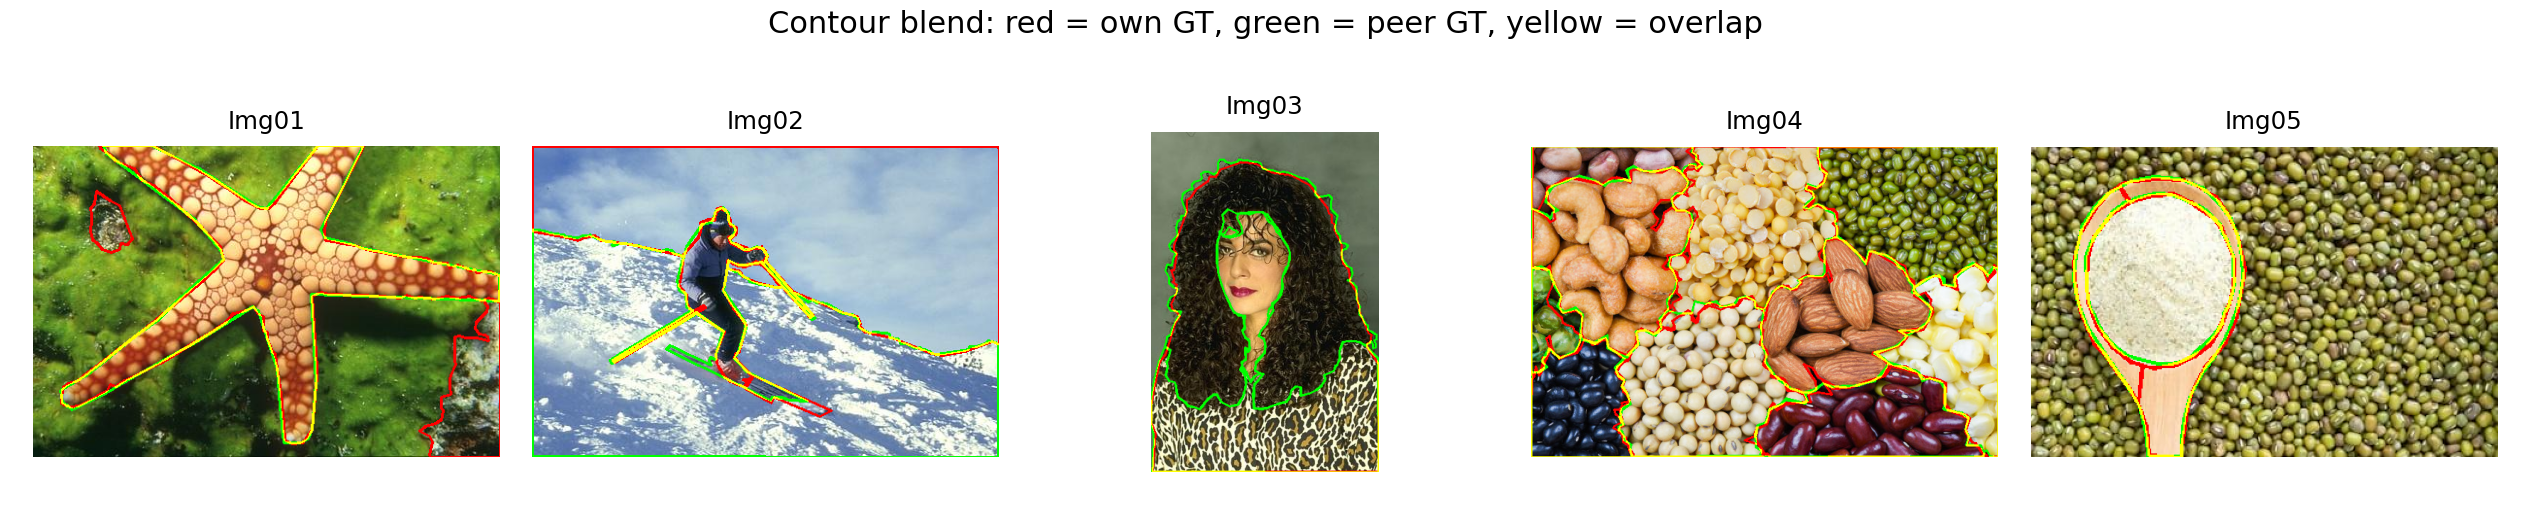
\includegraphics[width=0.95\textwidth,height=0.30\textheight,keepaspectratio]{figures/grids/peer_contour_blend_part1.png}
\caption{Self-vs-peer contour blends for Images 01--05. Red shows the self GT contour, green shows the peer GT contour, and yellow indicates overlap.}
\label{fig:peer-contour-blend-a}
\end{figure}
\begin{figure}[H]
\centering
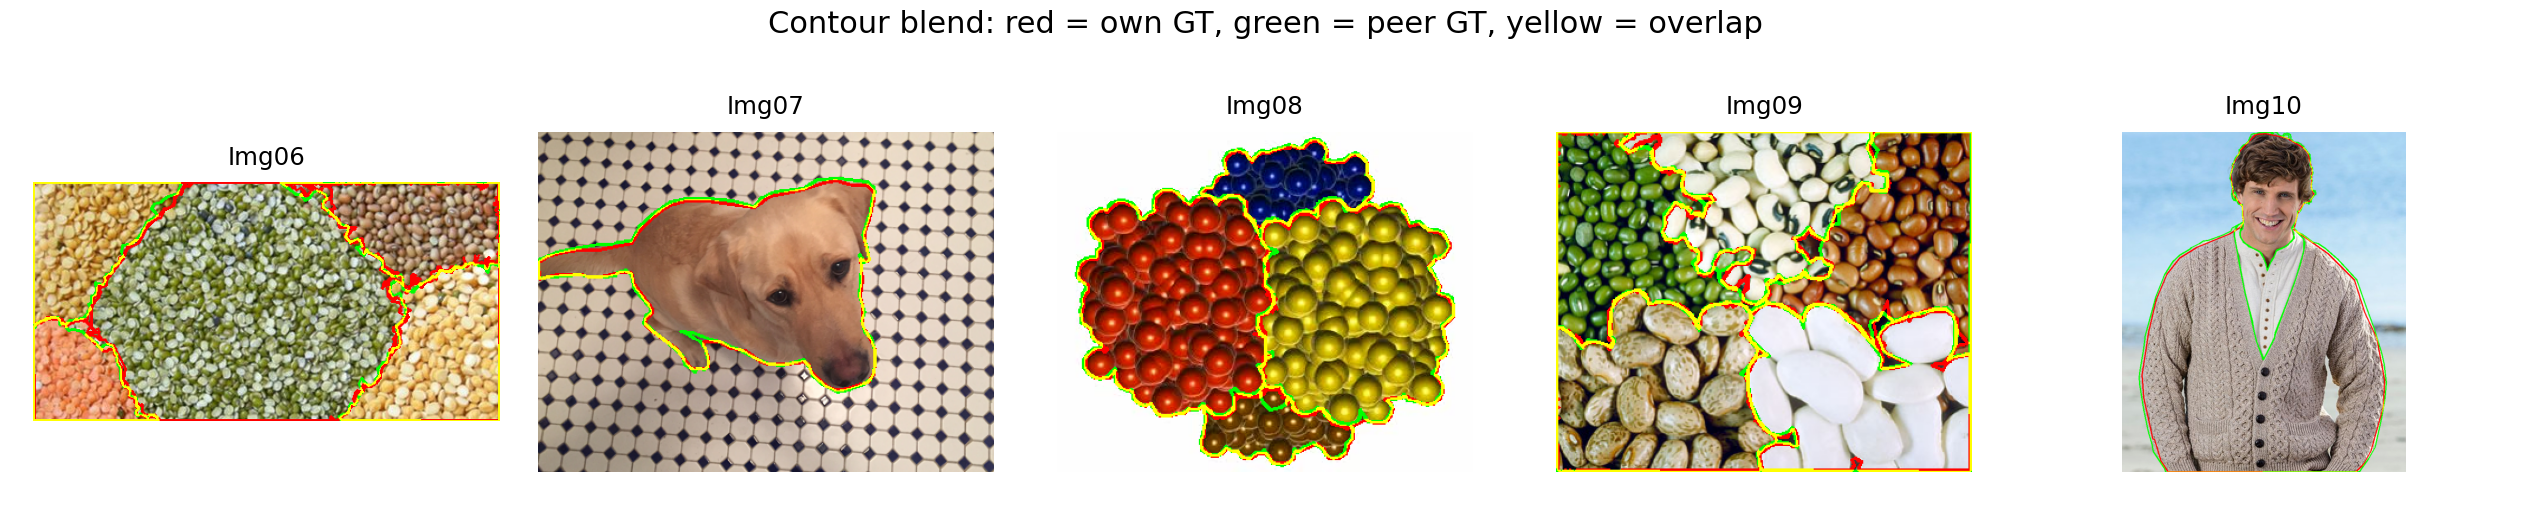
\includegraphics[width=0.95\textwidth,height=0.30\textheight,keepaspectratio]{figures/grids/peer_contour_blend_part2.png}
\caption{Self-vs-peer contour blends for Images 06--10.}
\label{fig:peer-contour-blend-b}
\end{figure}

\begin{figure}[H]
\centering
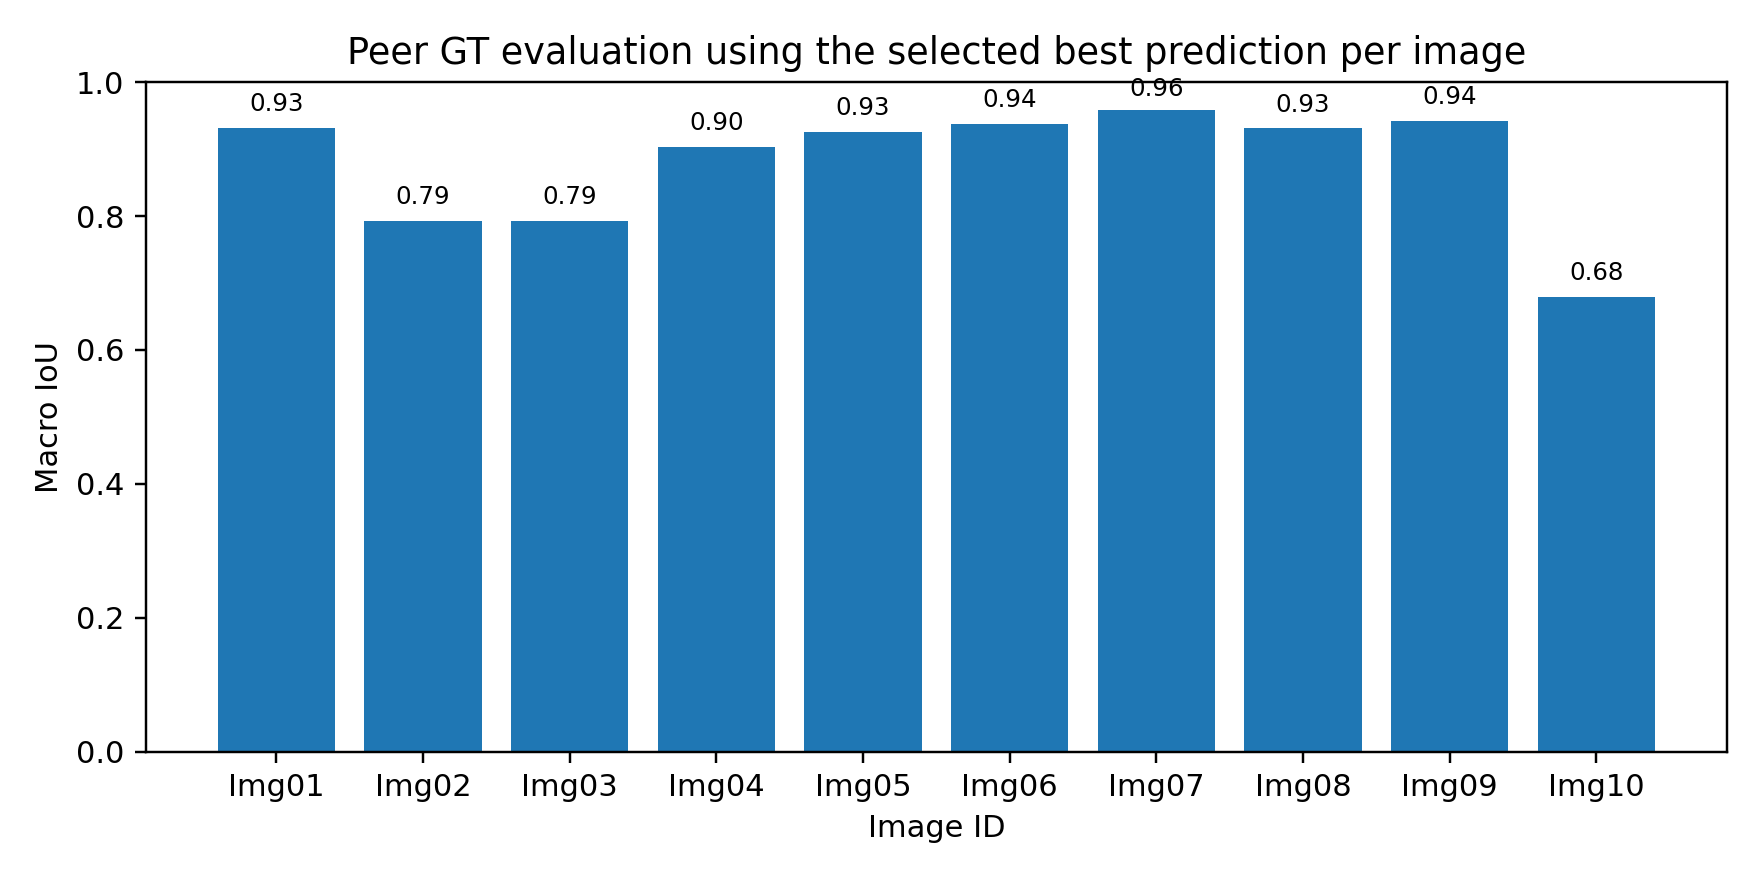
\includegraphics[width=0.82\textwidth]{figures/charts/peer_best_iou_by_image.png}
\caption{Macro IoU against peer GT using the selected best prediction per image.}
\label{fig:peer-iou}
\end{figure}

The peer-GT evaluation over ten images obtains macro Precision 0.958, macro Recall 0.917, macro IoU 0.880, and macro Boundary F1-score 0.681. The detailed per-image peer results are stored in \texttt{numerical\_results/peer\_gt/peer\_best\_per\_image\_results.csv}.

\begin{table}[H]
\centering
\caption{Peer-GT numerical results for the selected best prediction per image.}
\resizebox{\textwidth}{!}{%
\begin{tabular}{@{}lrrrrrr@{}}
\toprule
Image & Feature & Alg. & Prec. & Recall & IoU & BF \\
\midrule
Img01 & xy\_hsv & Mean Shift & 0.972 & 0.958 & 0.932 & 0.781 \\
Img02 & xy\_lab & Mean Shift & 0.945 & 0.836 & 0.793 & 0.532 \\
Img03 & hsv & Mean Shift & 0.924 & 0.856 & 0.793 & 0.344 \\
Img04 & xy\_lab & Mean Shift & 0.933 & 0.965 & 0.904 & 0.615 \\
Img05 & lab & Mean Shift & 0.953 & 0.970 & 0.926 & 0.904 \\
Img06 & xy\_lab & Mean Shift & 0.957 & 0.979 & 0.937 & 0.769 \\
Img07 & hsv & Mean Shift & 0.991 & 0.966 & 0.958 & 0.833 \\
Img08 & LAB\_XY & Mean Shift & 0.970 & 0.959 & 0.931 & 0.889 \\
Img09 & xy\_lab & Mean Shift & 0.961 & 0.980 & 0.942 & 0.778 \\
Img10 & xy\_hsv & Mean Shift & 0.971 & 0.706 & 0.680 & 0.361 \\
\bottomrule
\end{tabular}
}
\label{tab:peer-results}
\end{table}

The contour blend indicates that the largest disagreements usually occur at ambiguous boundaries or thin structures. This is expected because manual polygon annotations from two people rarely match perfectly. The high peer macro IoU still suggests that the selected segmentations are not merely overfitting one annotation set; they are broadly consistent with another GT interpretation.
